\documentclass{standalone}
\usepackage{tikz}
\usepackage{tikz-qtree}

\begin{document}

\tikzset{edge from parent/.style= {draw, edge from parent path={(\tikzparentnode.south) -- +(0,-8pt) -| (\tikzchildnode)}},
every node/.append style = {draw, circle, minimum size=20pt, inner sep=0pt, align=center, font=\sffamily\bfseries},
level 1/.style = {sibling distance=40pt, level distance=40pt},
level 2/.style = {sibling distance=20pt, level distance=40pt},
level 3/.style = {sibling distance=10pt, level distance=40pt}}

% draw a complete binary tree
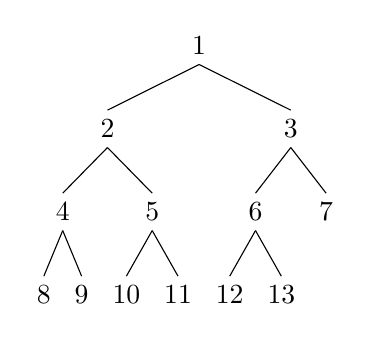
\begin{tikzpicture}
    \Tree [.1
        [.2 [.4 [.8 ] [.9 ] ] [.5 [.10 ] [.11 ] ] ]
        [.3 [.6 [.12 ] [.13 ] ] [.7 ] ] ]
    ]
\end{tikzpicture}

\end{document}